\documentclass[colorBG,slideColor,8pt]{beamer}
\mode<presentation>
{
  % Use the IIS-theme
  \usetheme{FHL}
  % Der mathematische Schriftsatz ist mit Serifen
  \usefonttheme[onlymath]{serif}
  % Noch nicht aufgedeckte Punkte erscheinen ausgegraut
%  \setbeamercovered{transparent}
  % Bild-/Tabellenüberschriften sind sehr klein
  \setbeamerfont{caption}{size=\tiny}
}

\usepackage[german]{babel}
\usepackage[utf8]{inputenc}
\usepackage{amsmath,bm}
\usepackage{accents}
\usepackage[]{easymovie}
\usepackage{lmodern}
\usepackage{helvet} 
\usepackage{setspace}
\renewcommand{\familydefault}{\sfdefault}

\usepackage{etoolbox}
\usepackage{booktabs}
\usepackage{tabulary}
\usepackage{multirow}

\usepackage[version-1-compatibility]{siunitx}
\sisetup{detect-family, locale=DE}

\usepackage{caption}
\captionsetup[figure]{name=}
\captionsetup[table]{name=}

\usepackage{subcaption}
\captionsetup[subfigure]{list=true, font=small, labelfont=bf, 
	labelformat=brace, position=bottom}

%
% Dick der Folientitel 1. Folie
%
\newcommand{\talktitle}{Evaluierung von Methoden zur Bestimmung der ventilatorischen Schwellen in der Spiroergometrie} 
%
% Some useful macros:
\newcommand{\MatDef}[2]{\left[ \hspace{-0.4em} \begin{array}{#1} #2 \end{array} \hspace{-0.4em} \right]}
\newcommand{\E}[1]{\ensuremath{\mathrm{E}\hspace{-0.12em}\left\{#1\right\}}}
\newcommand{\real}[1]{\ensuremath{\mathrm{Re}\hspace{-0.12em}\left\{#1\right\}}}
\newcommand{\imag}[1]{\ensuremath{\mathrm{Im}\hspace{-0.12em}\left\{#1\right\}}}
\newcommand{\ex}[1]{\ensuremath{e^{#1}}}
\newcommand{\rect}[1]{\ensuremath{\mathrm{rect}\left(#1\right)}}
\newcommand{\tri}[1]{\ensuremath{\mathrm{tri}\left(#1\right)}}
\newcommand{\mycos}[1]{\ensuremath{\cos{\left(#1\right)}}}
\newcommand{\mysin}[1]{\ensuremath{\sin{\left(#1\right)}}}
\newcommand{\corrbone}{\quad  \mbox{$\circ$  \hspace{-0.65em} --- \hspace{-0.65em}  $\bullet$}  \quad}
\newcommand{\invcorrbone}{\quad  \mbox{$\bullet$  \hspace{-0.65em} --- \hspace{-0.65em}  $\circ$}  \quad}
\newcommand{\maker}[1]{\textcolor{red!80!black}{#1}}
\newcommand{\makeg}[1]{\textcolor{green!74!black}{#1}}
\newcommand{\makeb}[1]{\textcolor{blue!80!black}{#1}}
\newcommand{\eqotwo}{EQO\textsubscript{2}}
\newcommand{\eqcotwo}{EQCO\textsubscript{2}}
\newcommand{\votwo}{\.{V}O\textsubscript{2}}
\newcommand{\vcotwo}{\.{V}CO\textsubscript{2}}
\newcommand{\ve}{\.{V}E}

% Literaturverzeichnis:
\usepackage[autostyle=true,german=quotes]{csquotes}
\usepackage[
backend=biber,
style=iso-authoryear,
autolang=other,
bibencoding=UTF8,
maxnames=3,
hyperref
]{biblatex}

\DefineBibliographyStrings{ngerman}{andothers={et\ al\adddot}}
\addbibresource{Referenzen.bib}

\AtBeginSection[]{
		\frame{
		\frametitle{}
		\tableofcontents[currentsection]
		}
}

\apptocmd{\UrlBreaks}{\do\f\do\m}{}{}
\setcounter{biburllcpenalty}{9000}% Kleinbuchstaben
\setcounter{biburlucpenalty}{9000}% Großbuchstaben
%
% -----------------------------------------------------------
% Begin
% -----------------------------------------------------------
\begin{document}
% -----------------------------------------------------------
% Title page
% -----------------------------------------------------------
\begin{frame}
    \vspace{-10ex}
    \textcolor{fhlred}{\HRuleFill[0.4ex]} \\ \vspace{1ex}
    {\linespread{1.5}\selectfont
    \MakeUppercase{\bf \huge \talktitle}\\[5.5ex]}
    \normalsize Kolloquium zur Bachelorthesis\\
    \textcolor{fhlred}{\HRuleFill[0.1ex]} \\ \vspace{4ex}
    \small Julian-Marvin Lütten\\
    \small Fachschule Lübeck, B.Sc. Biomedizintechnik\\
    \vspace{2ex}
    \small angefertigt bei der\\
    \small cardioscan GmbH\\
    \small 2018
\end{frame}

\begin{frame}{Inhalt}
\tableofcontents
\end{frame}

% -----------------------------------------------------------
% Kapitel 1: Relevanz des Themas
% -----------------------------------------------------------

\section{Relevanz des Themas}

\begin{frame}
\begin{itemize}
	\item 14,4 \% Anstieg der Mitgliederzahl in deutschen Fitnessstudios zwischen 2014 und 2017\\größter Sektor: Gesundheit \& Prävention~(\cite{DSSV.2018}) = Hauptabnehmer der cardioscan GmbH
	\item cardioscan bietet u.a. Spiroergometrie an (bisher mit Dritthersteller-Geräten und eigener \textsl{cardioscan Checkpoint Software (CCPS)})
	\item Zweck: Definition von individuellen Trainingsbereichen
	\item neues Spiroergometer \textsl{metabolicscan} soll künftige Hardware darstellen
	\item Stand der Forschung: Detektion von Stoffwechselübergängen durch Bestimmung der ventilatorischen Schwellen~(\cite{Westhoff.2012})
	\item veralteter Software-Algorithmus: VT2 $\hat{=}$  RQ $=$ 1 ist akut beeinflussbar\\$\rightarrow$ anfällig für Fehler und wissenschaftlich umstritten
\end{itemize}
\end{frame}

% -----------------------------------------------------------
% Kapitel 2: Ventilatorisches Schwellenkonzept
% -----------------------------------------------------------

\section{Ventilatorisches Schwellenkonzept}

\begin{frame}
\begin{itemize}
	\item inkrementierte körperliche Arbeit $\rightarrow$ erhöhter Energiebedarf $\rightarrow$ metabolische Reaktion: Stoffwechselumstellungen: aerob $\rightarrow$ aerob-anaerob $\rightarrow$ anaerob
	\item erhöhte Glykolyse-Rate $\rightarrow$ Laktatproduktion $\rightarrow$ metabolische Azidose $\rightarrow$ anfallendes CO\textsubscript{2} $\rightarrow$ messbare Zunahme der \vcotwo{} und \ve
	\item Messung der Atemgase in festen Abständen $\rightarrow$ grafische Darstellung der Parameter
	\item von AG Spiroergometrie werden einige Methoden empfohlen (\cite{Westhoff.2012})
	\item Bestimmung der ventilatorischen Schwellen mit jeweils zwei ausgewählten Methoden (VT1: V-Slope, \eqotwo; VT2: \eqcotwo, \ve/\vcotwo)
\end{itemize}
\begin{columns}
\begin{column}{\linewidth}
\begin{figure}[H]
	\begin{subfigure}[c]{0.2\linewidth}
		\centering
		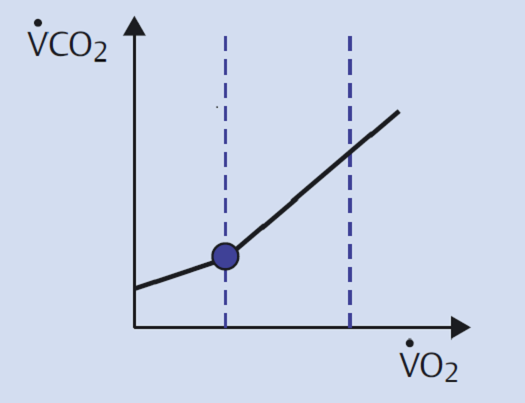
\includegraphics[width=0.8\linewidth]{Bilder/vslope.png}
		\subcaption{V-Slope}
	\end{subfigure}
	\begin{subfigure}[c]{0.2\linewidth}
		\centering
		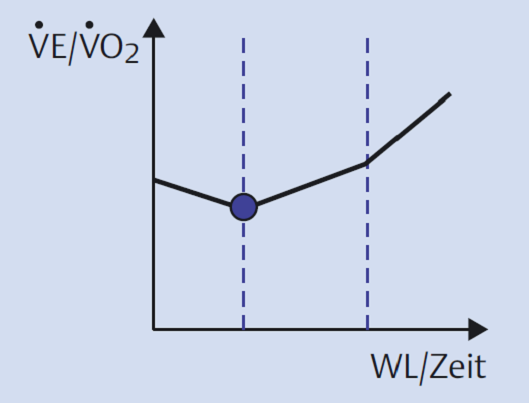
\includegraphics[width=0.8\linewidth]{Bilder/eqo2.png}
		\subcaption{\eqotwo}
	\end{subfigure}
	\begin{subfigure}[c]{0.2\linewidth}
		\centering
		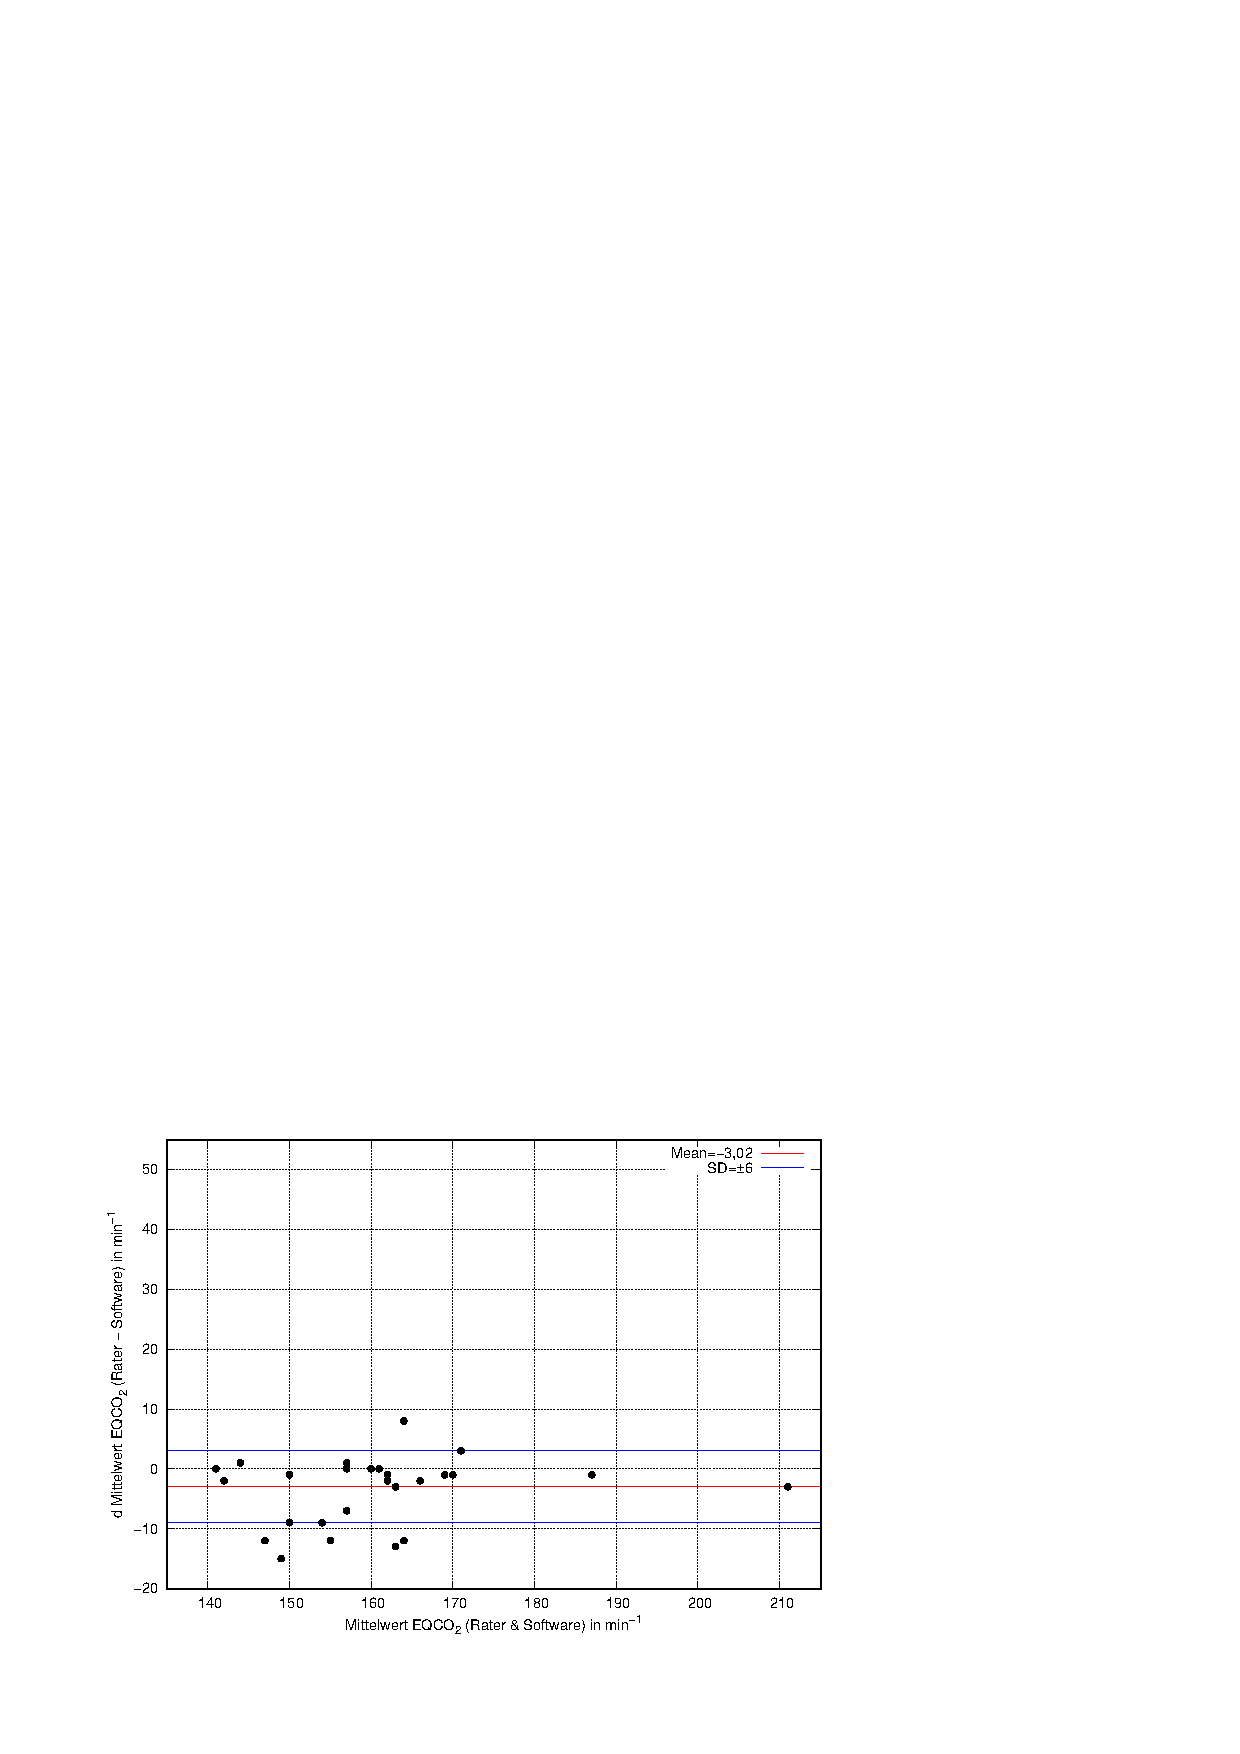
\includegraphics[width=0.8\linewidth]{Bilder/eqco2.png}
		\subcaption{\eqcotwo}
	\end{subfigure}
	\begin{subfigure}[c]{0.2\linewidth}
		\centering
		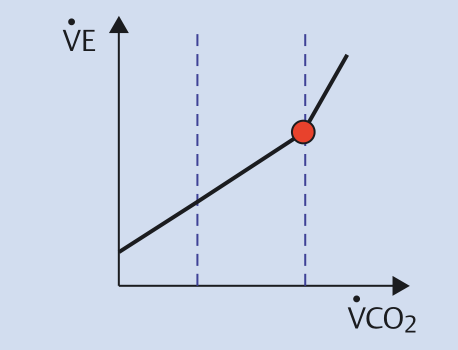
\includegraphics[width=0.8\linewidth]{Bilder/field4.png}
		\subcaption{\ve/\vcotwo}
	\end{subfigure}
\end{figure}
\end{column}
\end{columns}
\end{frame}

% -----------------------------------------------------------
% Kapitel 3: Herausforderung und Aufgabenstellung
% -----------------------------------------------------------

\section{Herausforderungen und Aufgabenstellung}

\begin{frame}
\begin{block}{Unternehmensziele}
	\begin{itemize}
		\item optimale Methode zur Schwellenbestimmung für optimierten Algorithmus erarbeiten
		\item neue Basis für eine zuverlässigere Definition der Trainingsbereiche erstellen
	\end{itemize}
\end{block}
\begin{block}{Forschungsfragen}
	\begin{enumerate}
		\item Eignet sich der metabolicscan zur Durchführung einer Spiroergometrie?
		\item Mit welcher Methode können die Schwellen optimal bestimmt werden?
		\item Ist eine genauere Bestimmung der VT2 mit den neuen Methoden möglich?
	\end{enumerate}
\end{block}
\end{frame}

% -----------------------------------------------------------
% Kapitel 3: Methoden
% -----------------------------------------------------------
\section{Methoden}

\begin{frame}{Testprojekt}
\begin{itemize}
	\item spiroergometrische Testmessungen mit 28 internen und externen Probanden unter gleichen Bedingungen (Temp. zwischen \SI{18}{\degreeCelsius} und \SI{22}{\degreeCelsius} etc.)
	\item Personen zwischen 18 und 60 Jahren, Sportler und Nicht-Sportler, Raucher und Nichtraucher
	\item Anamnesegespräch + Ruhe-EKG + Bestimmung der ungefähren Soll-Belastung und des individuellen Belastungsprotokolls
	\item Leerlastphase $\rightarrow$ Ruhestoffwechselmessung $\rightarrow$ Belastungsphase
	\item Speichern der Rohdaten in CSV-Dateien
	\item Weiterverarbeitung + Auswertung der Rohdaten durch MATLAB-Programm
	\item Schwellenbestimmung: manuell durch zwei Rater + algorithmisch
	\item Vergleich mit Referenzstudie HUNT 3 (\cite{Loe.2014})
\end{itemize}
\end{frame}

\begin{frame}{Funktionsweise des metabolicscan}
\begin{columns}
\begin{column}{0.5\linewidth}
\begin{itemize}
	\item Modularer Aufbau: Atemmodul mit Flowsensor + Analysemodul mit CO\textsubscript{2}/O\textsubscript{2}-Sensormodul
	\item Atemmodul: Messung der Strömungsgeschwindigkeit der Inspirations- und Exspirationsluft
	\item Berechnung des Strömungsvolumens durch mathematische Integration über die Zeit
	\item Pumpe saugt Luftanteil durch Probenschlauch zum Analysemodul
	\item CO\textsubscript{2}-Messung durch Infratotlichtabsorption
	\item Weiterleitung zum galvanischen O\textsubscript{2}-Sensor
\end{itemize}
\end{column}
\begin{column}{0.5\linewidth}
			\begin{figure}[H]
				\centering
				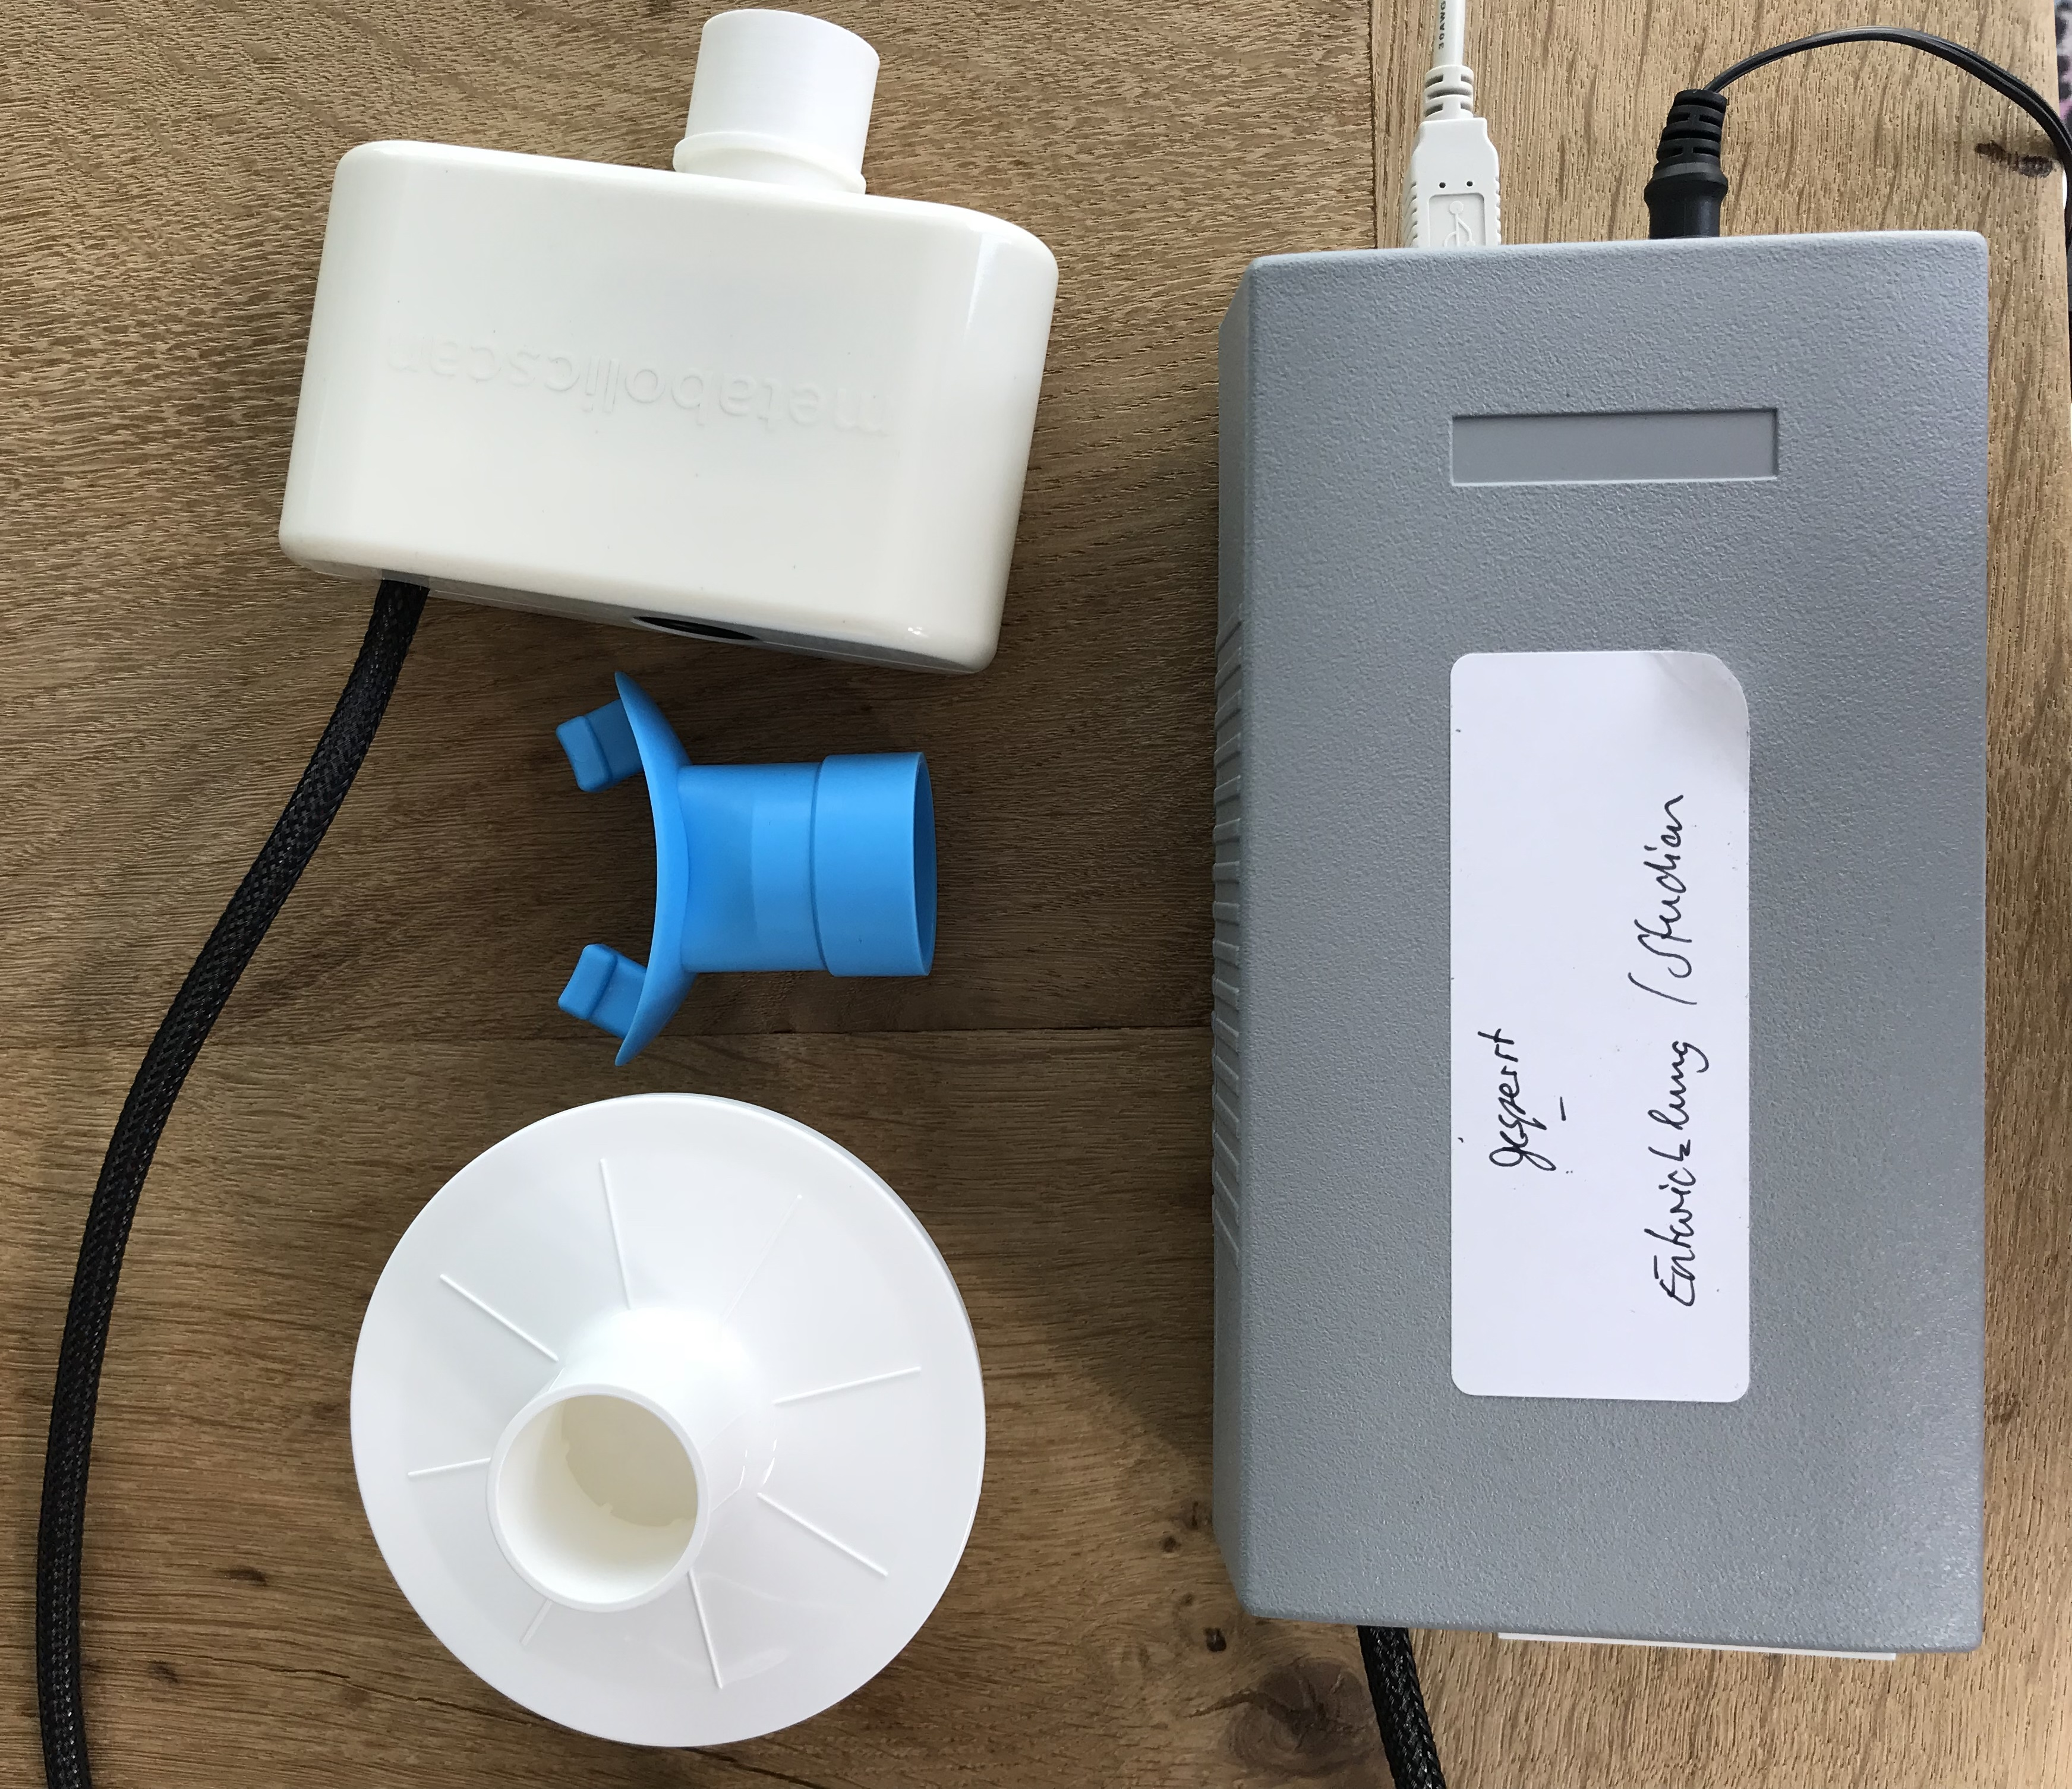
\includegraphics[width=0.8\linewidth]{Bilder/mbs.jpg}
				\caption{metabolicscan: Analysemodul, Atemmodul, Filter und Mundstück}
			\end{figure}
\end{column}
\end{columns}
\end{frame}

% -----------------------------------------------------------
% Kapitel 4: Resultate
% -----------------------------------------------------------
\section{Resultate}

\begin{frame}{"`6-Felder-Grafiken"'}
\begin{columns}
	\begin{column}{0.5\linewidth}
		\begin{itemize}
			\item Keine Störungen oder Fehler während der Messungen
			\item "`6-Felder-Grafiken"' für jeden Probanden generiert: eine für manuelle Bestimmung, eine mit algorithmischen Schwellenbestimmungen
			\item teilweise nicht-differenzierbare Plots; vorwiegend bei den VT1-Methoden
			\item Differenzen zwischen den einzelnen Ergebnissen der Rater und Software\\$\rightarrow$ statistische Auswertung
		\end{itemize}
	\end{column}
	\begin{column}{0.5\linewidth}
		\begin{figure}[H]
			\centering
			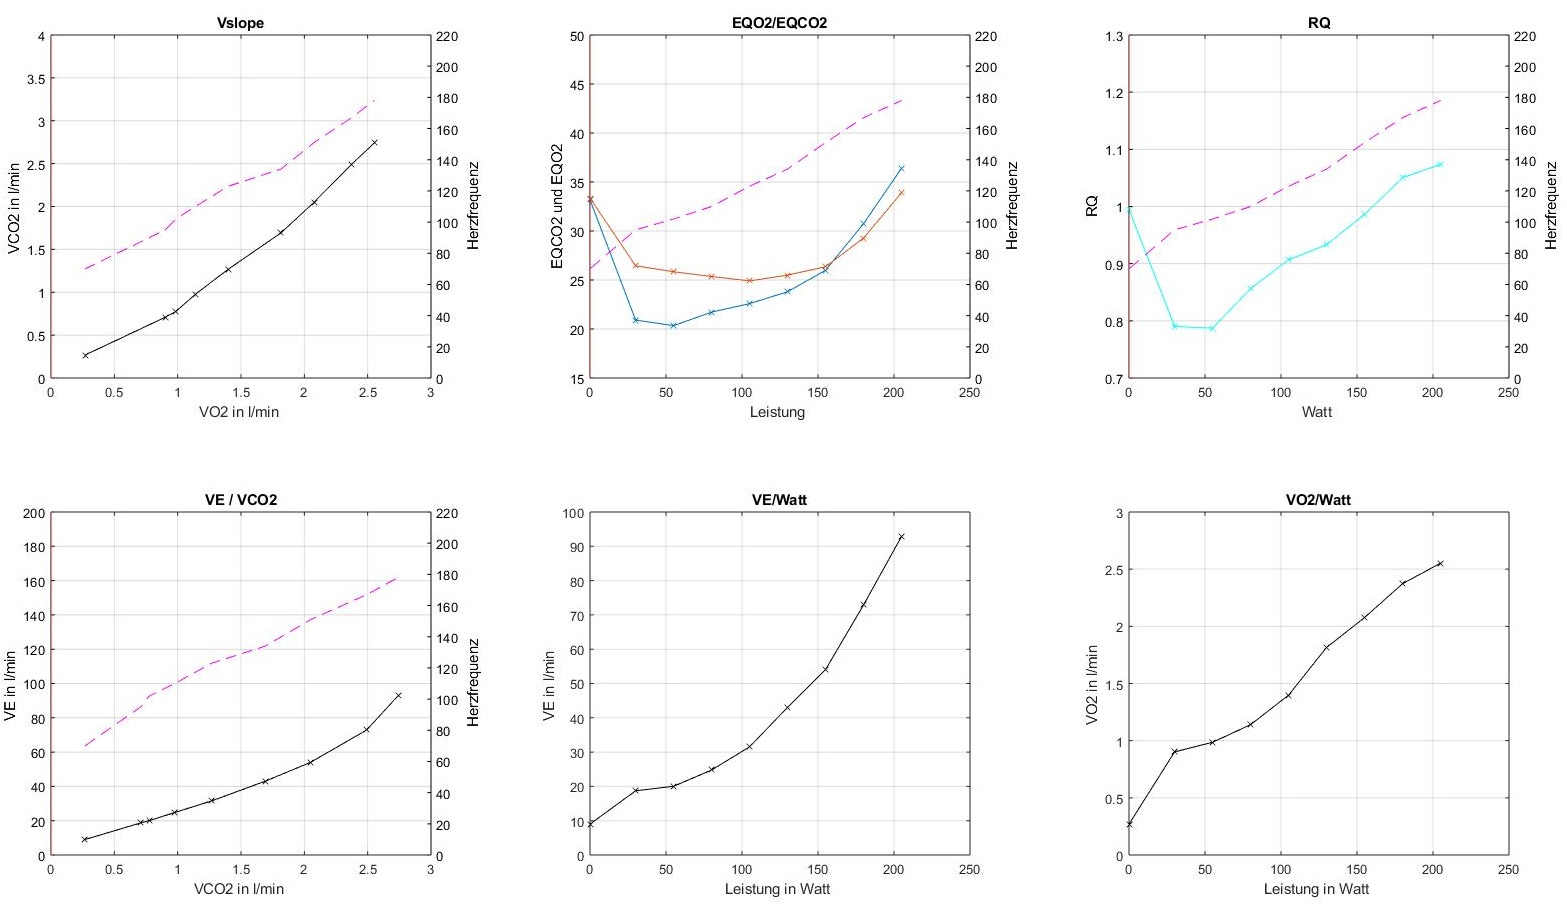
\includegraphics[width=0.8\linewidth]{Bilder/plot_6w.jpg}
			\caption{Manuell}
			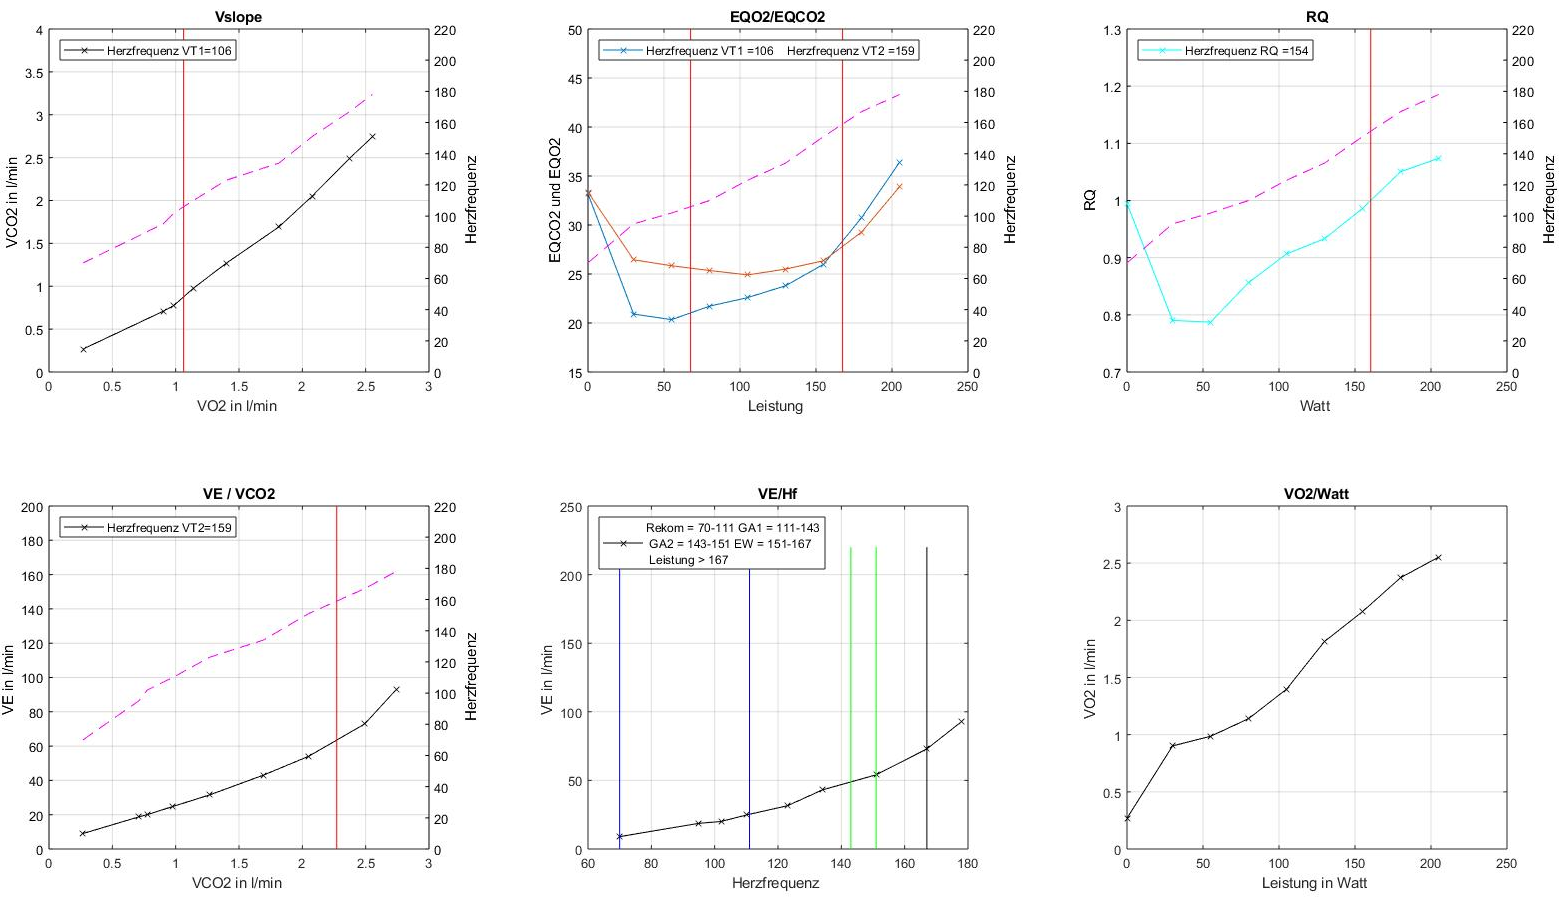
\includegraphics[width=0.8\linewidth]{Bilder/auto_6.png}
			\caption{Algorithmisch}
		\end{figure}
	\end{column}
\end{columns}
\end{frame}

\begin{frame}[fragile]{VT1-Ergebnisse}
\begin{columns}
	\begin{column}{0.5\linewidth}
		\begin{figure}
			\begin{subfigure}{0.9\linewidth}
				\centering
				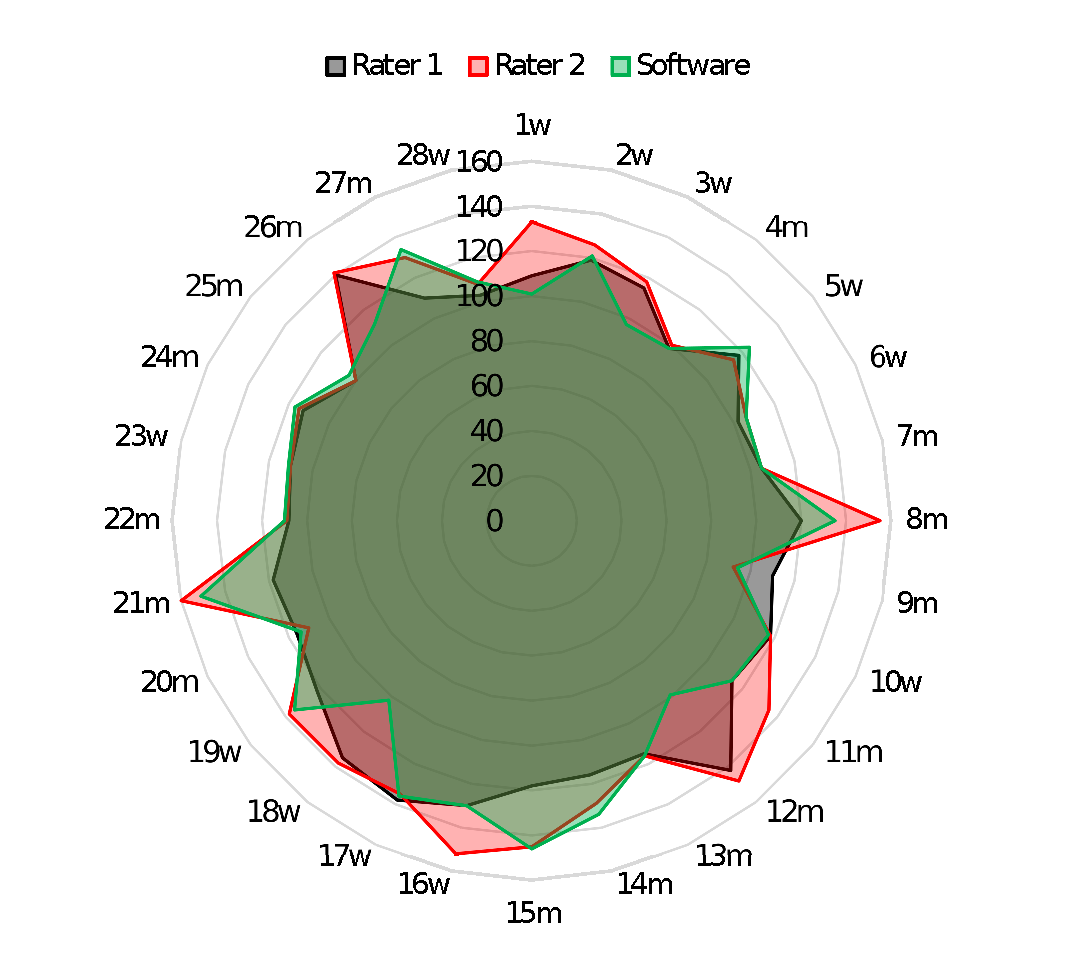
\includegraphics[width=0.6\linewidth]{Bilder/v-slope_net.eps}
			\end{subfigure}
			\begin{subfigure}{0.9\linewidth}
				\centering
				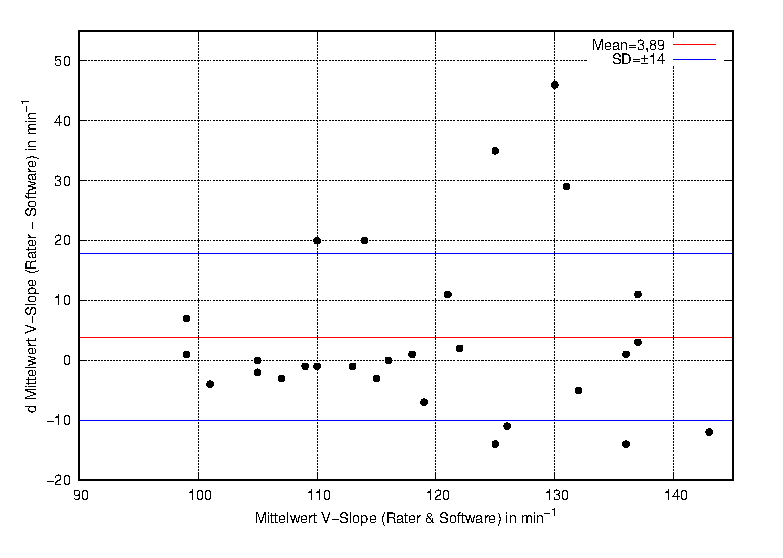
\includegraphics[width=0.82\linewidth]{Bilder/vslope.eps}
			\end{subfigure}	
			\caption{V-Slope}	
		\end{figure}
	\end{column}
	\begin{column}{0.5\linewidth}
		\begin{figure}
			\begin{subfigure}{0.9\linewidth}
				\centering
				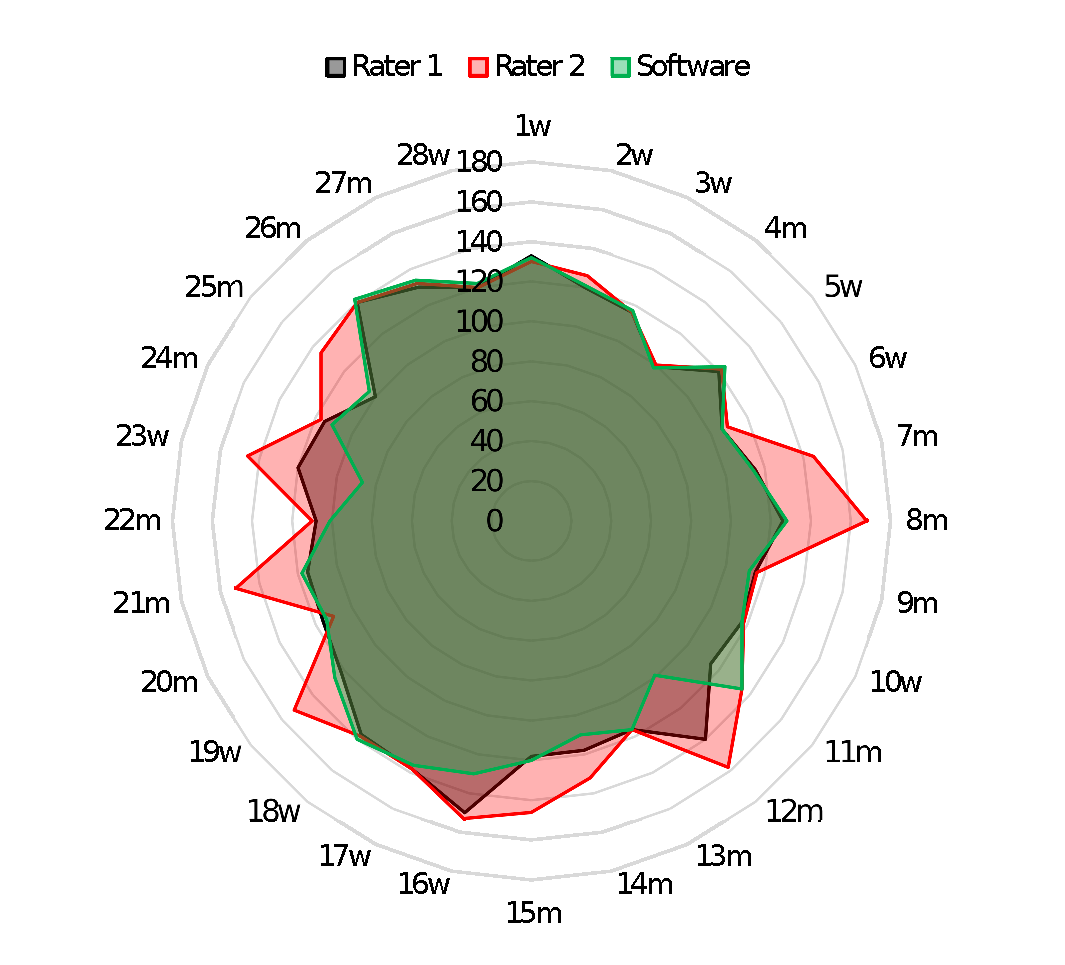
\includegraphics[width=0.6\linewidth]{Bilder/eqo2_net.eps}
			\end{subfigure}
			\begin{subfigure}{0.9\linewidth}
				\centering
				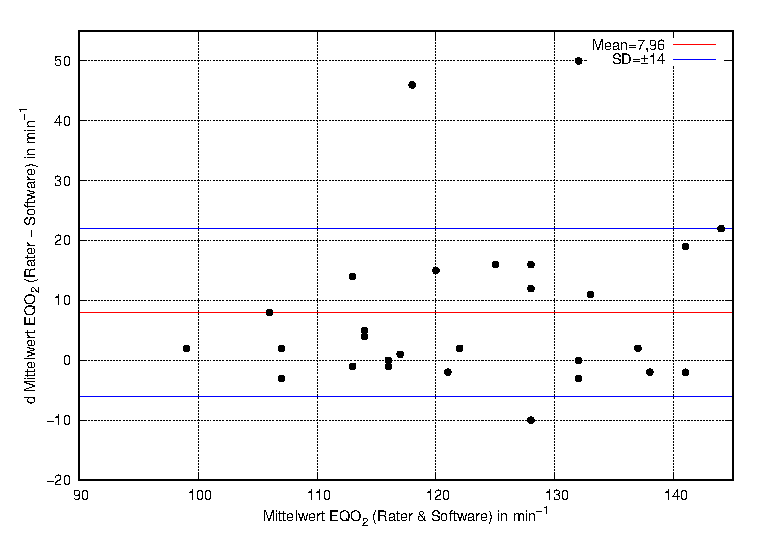
\includegraphics[width=0.82\linewidth]{Bilder/eqo2.eps}
			\end{subfigure}	
			\caption{\eqotwo}
		\end{figure}
	\end{column}
\end{columns}
\end{frame}

\begin{frame}[fragile]{VT2-Ergebnisse}
\begin{columns}
	\begin{column}{0.5\linewidth}
		\begin{figure}
			\begin{subfigure}{0.9\linewidth}
				\centering
				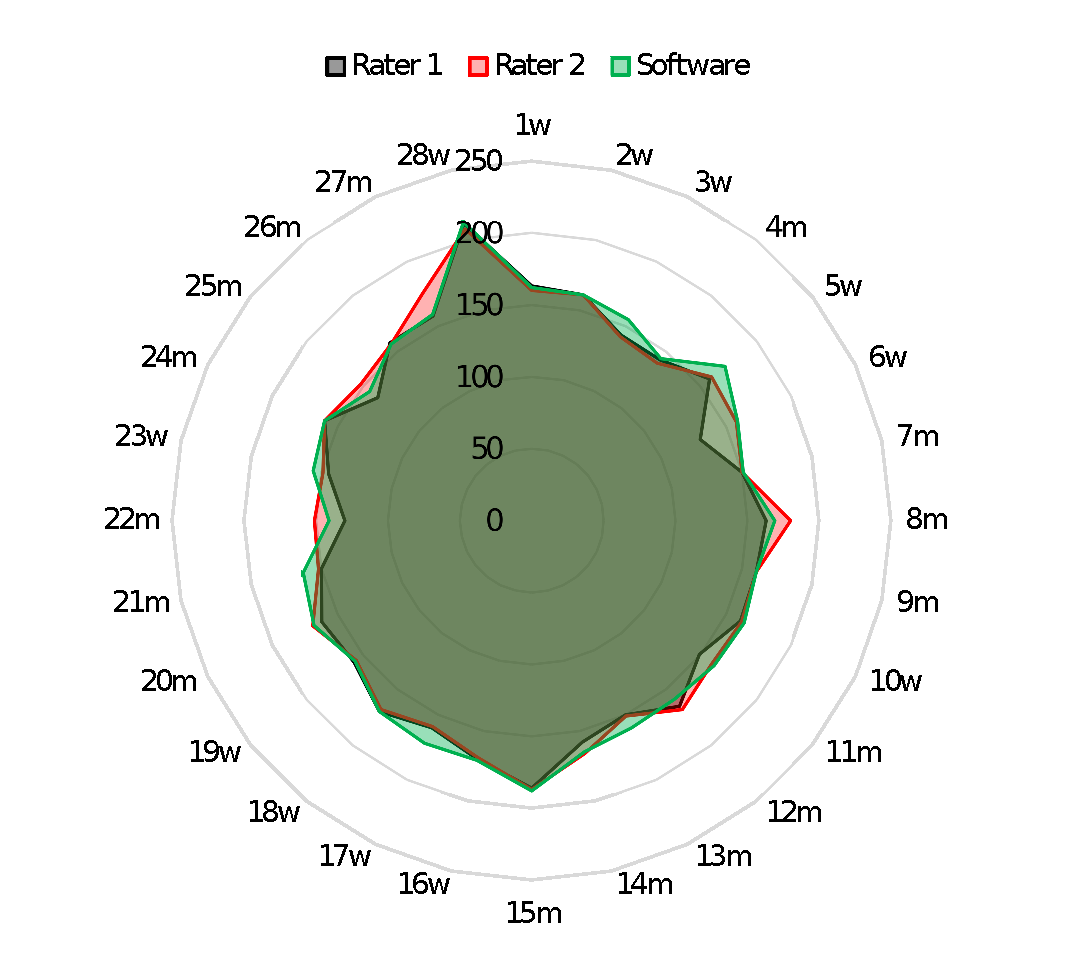
\includegraphics[width=0.6\linewidth]{Bilder/eqco2_net.eps}
			\end{subfigure}
			\begin{subfigure}{0.9\linewidth}
				\centering
				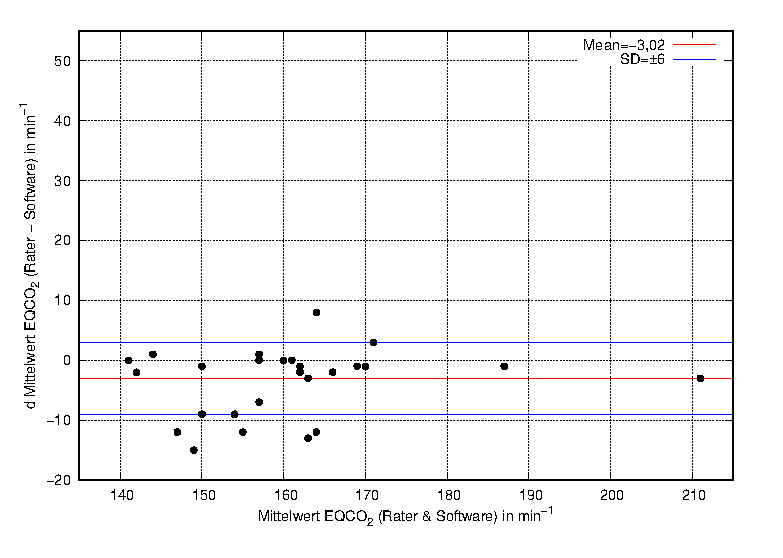
\includegraphics[width=0.82\linewidth]{Bilder/eqco2.eps}
			\end{subfigure}	
		\caption{\eqcotwo}	
		\end{figure}
	\end{column}
	\begin{column}{0.5\linewidth}
		\begin{figure}
			\begin{subfigure}{0.9\linewidth}
				\centering
				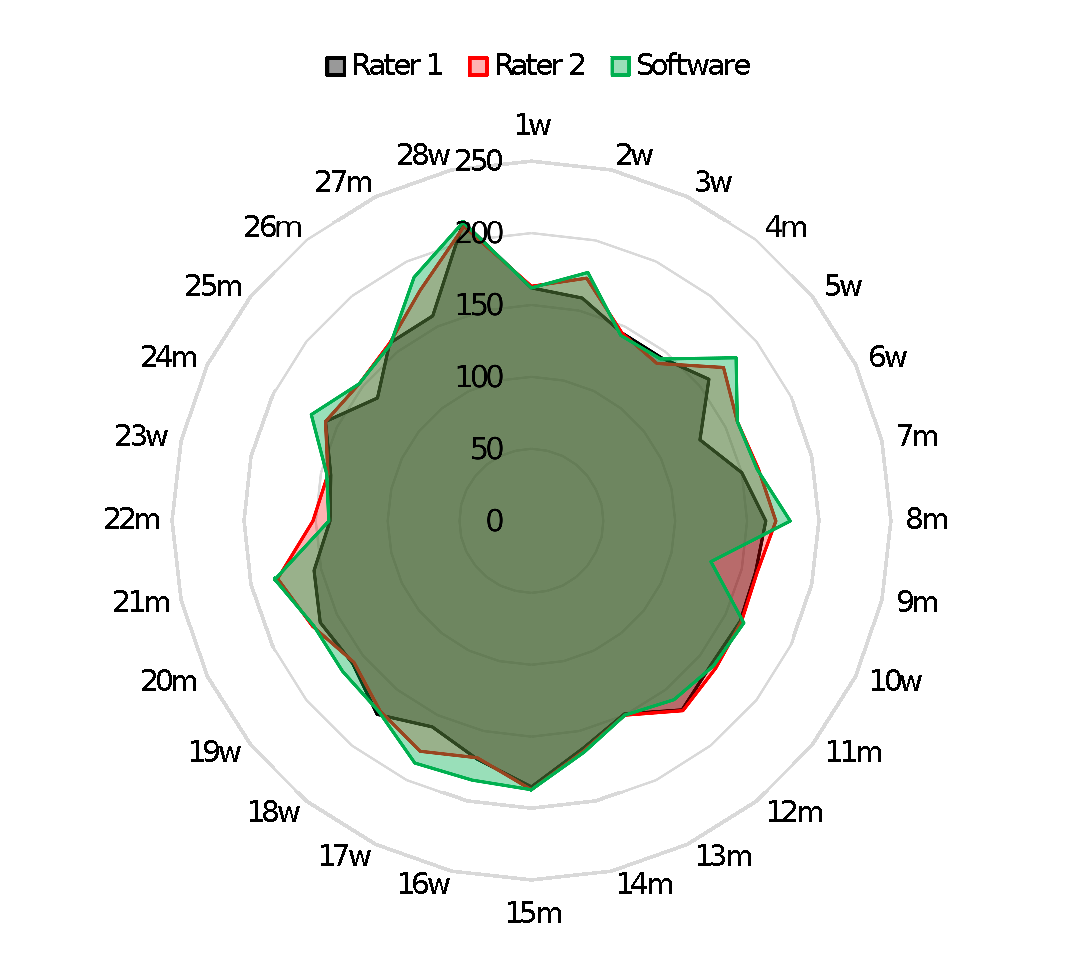
\includegraphics[width=0.6\linewidth]{Bilder/vevco2_net.eps}
			\end{subfigure}
			\begin{subfigure}{0.9\linewidth}
				\centering
				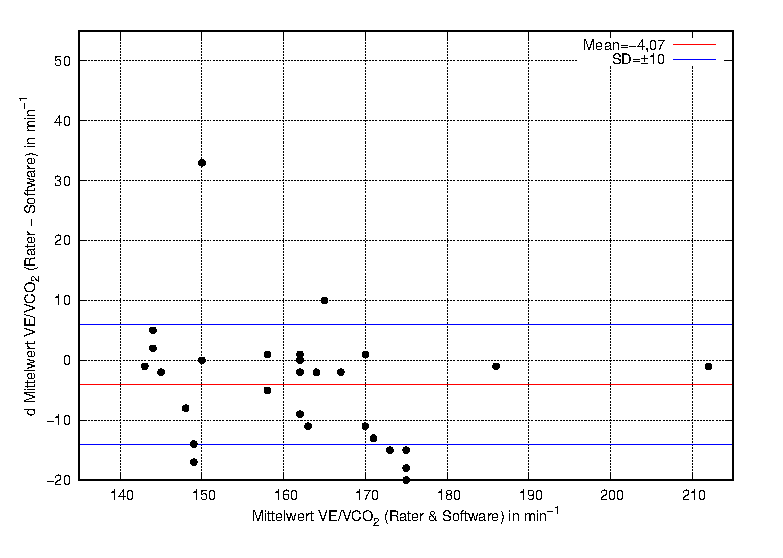
\includegraphics[width=0.82\linewidth]{Bilder/vevco2.eps}
			\end{subfigure}	
		\caption{\ve/\vcotwo}
		\end{figure}
	\end{column}
\end{columns}
\end{frame}

% -----------------------------------------------------------
% Kapitel 5: Diskussion
% -----------------------------------------------------------
\section{Diskussion}

\begin{frame}{Evaluation der Tests}
\begin{itemize}
	\item kritische Plots bzw. Schwankungen in den ersten Stufen $\rightarrow$ VT1-Bestimmung erschwert (siehe Differenzen der Ergebnisse)
	\item Analyse der Felder 5 und 6: Plausibilitätsprüfung des Verlaufs der \.{V}E bzw. der \.{V}CO\textsubscript{2} zur W\\$\rightarrow$ Annahme: idealerweise lineare Zunahme~(\cite{Ruehle.2012})
	\item Erkenntnis: Schwankungen zurückzuführen auf Fehler im Algorithmus bei Berechnung der Atemfrequenz
	\item neue Messungen bzw. eine erneute Auswertung könnte veränderte Ergebnisse liefern
	\item für alle Testmessungen konnten charakteristische Graphen generiert werden
	\item alle erhobenen Messwerte lagen innerhalb der Genauigkeitsgrenzen der Sensoren
\end{itemize}
\begin{center}
\vspace{3ex}
$\rightarrow$ Hypothese: Der metabolicscan kann für die Spiroergometrie genutzt werden.
\end{center}
\end{frame}

\begin{frame}{Evaluation der Methoden}
\begin{columns}
\begin{column}{0.5\linewidth}
\begin{figure}[H]
	\centering
	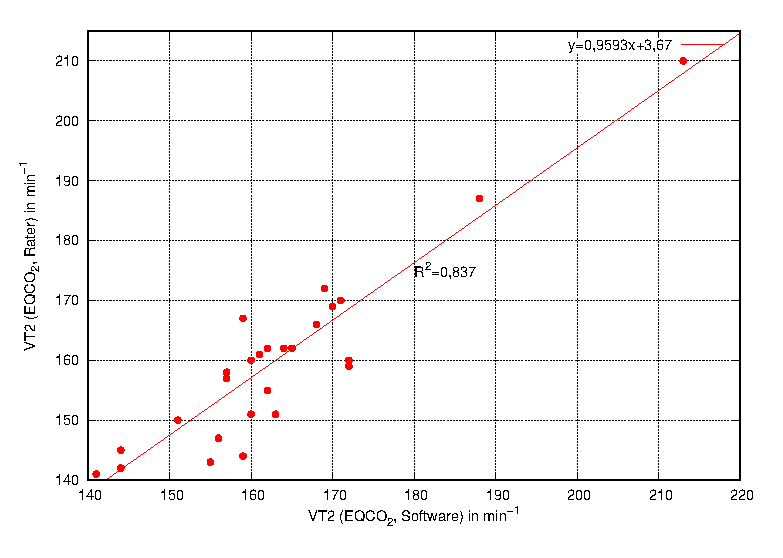
\includegraphics[width=\linewidth]{Bilder/korr_eqco2.eps}
	\caption{Regressionsanalyse der \eqcotwo-Ergebnisse}
\end{figure}
\end{column}
\begin{column}{0.5\linewidth}
	\eqcotwo{} ist die Methode mit den geringsten Abweichungen $\rightarrow$ optimale Methode\\
	\vspace{3ex}
	Korrelationskoeffizient $r = 0,912$\\
	\vspace{3ex}
	\ve/\vcotwo{} als geeignete Referenzmethode mit $r = 0,816$
\end{column}
\end{columns}
\end{frame}

\begin{frame}{Evaluation der Methoden}
\begin{itemize}
	\item V-Slope-Plots häufig nicht differenzierbar $\rightarrow$ fehlerhafter Algorithmus zur Bestimmung der Atemfrequenz (AF) $\rightarrow$ viele Differenzen: $r = 0,526$
	\item Schwankungen der \eqotwo-Kurve bzw. kein eindeutiger Tiefpunkt $\rightarrow$ häufiger große Differenzen zwischen den Ergebnissen: $r = 0,464$
	\item mit einem Modell nach W. Kindermann ist die Trainingszonendefinition nur von VT2 abhängig (\cite{Kindermann.2004}) $\rightarrow$ VT1 zum Erreichen des Zieles nicht zwingend erforderlich
	\item 9 von 28 Tests mit RQ=1-Methode nicht auswertbar; bei auswertbaren Plots: häufig hohe Differenzen zu anderen Methoden
	\item Vergleich mit HUNT 3: 15 von 28 Ergebnissen befinden sich innerhalb des altersspezifischen Durchschnitts (trotz unterschiedlicher Belastungsprotokolle)
\end{itemize}
\end{frame}

\begin{frame}{Fazit \& Handlungsempfehlung}
\begin{itemize}
	\item mit \eqcotwo{} wurde eine genauere Methode zur VT2-Bestimmung erarbeitet
	\item mit dieser Methode können realistische Trainingszonen nach dem Modell von Kindermann definiert werden
	\item der Software-Algorithmus zur grafischen Verarbeitung sollte noch weiter optimiert werden
	\item Mittelung der Messwerte über die Gesamtanzahl der Atemzüge pro Stufe wegen des Algorithmusfehlers problematisch $\rightarrow$ evtl. Alternative: gleitende Mittelung
	\item Alternativen zum Mundstück könnten Atmung des Probanden optimieren/erleichtern\\$\rightarrow$ evtl. Reduktion von Messfehlern
	\item einige Einflussfaktoren sind bei der Durchführung zu beachten: probandenbedingt, anwenderbedingt, umweltbedingt\\$\rightarrow$ Produkt- und Konzept-Schulungen durch cardioscan Academy sind wichtig
	\item \eqcotwo-Algorithmus wird in die CCPS implementiert
\end{itemize}
\end{frame}

\begin{frame}
\begin{center}
	\large{\textbf{Vielen Dank für Ihre Aufmerksamkeit!}}
\end{center}
\end{frame}

% -----------------------------------------------------------
% Kapitel 6: Literatur
% -----------------------------------------------------------
\section{Literatur}

\begin{frame}
\begin{columns}
\begin{column}{0.9\linewidth}
\nocite{*}
\printbibliography
\end{column}
\end{columns}
\end{frame}

\end{document}